% !TeX root = main.tex

Los Merkle Trees tradicionales permiten realizar pruebas eficientes de pertenencia a un conjunto de datos finito. Pero hay una limitación fundamental a la hora de realizar pruebas de exclusión, es decir de la \textbf{no pertenencia} de un dato $\ell$ a un conjunto $L$. En un Merkle Tree clásico, las hojas corresponden exclusivamente a los elementos de $L$. Una posible solución sería definir un orden total sobre $L$ (si fuera posible), construyendo una prueba de exclusión mostrando que el elemento consultado se encuentra entre dos hojas consecutivas del árbol. Observamos que en protocolos criptográficos esto no es ideal, pues se debe revelar información adicional sobre elementos vecinos en $L$. Para superar estas limitaciones se introducen los Sparse Merkle Trees.

\begin{definition}[Sparse Merkle Tree]
	Sean $k, n \in \mathbb{N}$, y $\mathcal{H}$ una función de hash criptográfica. Sea $D = \{0,1\}^k$ el dominio completo de posibles elementos (cadenas de $k$ bits). Dado $L \subseteq D$, un Sparse Merkle Tree $\mathcal{T}_{L,\mathcal{H}} = \mathcal{T}$ de altura $k$ y conjunto de datos almacenados $L$ es un árbol binario definido recursivamente de la siguiente manera:
	\begin{enumerate}
		\item Hojas: Cada elemento $x \in D$ se asocia en forma ordenada a una hoja $h_x$ de la siguiente forma:
		$$h_x = \begin{cases}
		\mathcal{H}(x), \text{ si } x \in L \\
		\mathcal{H}(\bot), \text{ si } x \not\in L
		\end{cases}$$
		donde $\bot \in D$ es un valor por defecto, predefinido y constante (default hash).
		\item Cada nodo interno $N$ con hijos $N_i$ (nodo hijo izquierdo) y $N_d$ (nodo hijo derecho) se define como $N = \mathcal{H}(N_i \Vert N_d)$.
		\item Es el nodo que sintetiza criptográficamente toda la información de $L$ sobre el dominio $D$.
		\item Aunque conceptualmente $\mathcal{T}$ tiene $2^k$ hojas, en la práctica solo se almacenan y calculan los nodos necesarios para representar los elementos de $L$ y los hashes por defecto de las ramas no ocupadas. Esto permite mantener las pruebas de pertenencia y exclusión de tamaño $O(k)$.
	\end{enumerate}
\end{definition}

\begin{figure}[h]
	\centering
	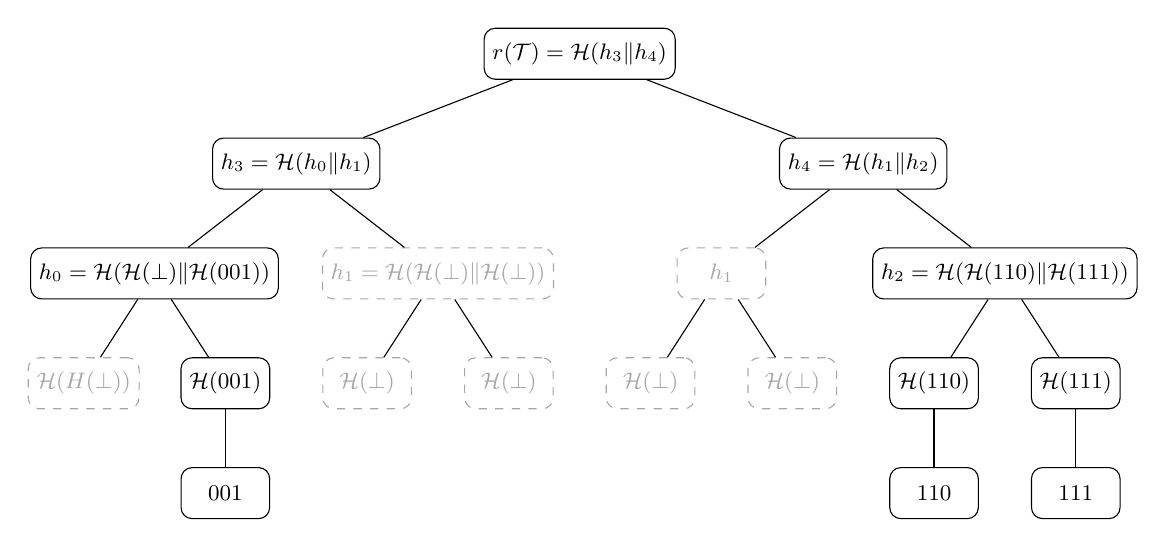
\begin{tikzpicture}[
		scale=0.9,
		transform shape,
		level distance=1.55cm,
		level 1/.style={sibling distance=8cm},
		level 2/.style={sibling distance=4cm},
		level 3/.style={sibling distance=2cm},
		every node/.style={
			draw, rectangle, rounded corners,
			align=center,
			minimum width=1.25cm,
			minimum height=0.72cm,
			font=\small
		},
		stored/.style={draw, opacity=1},
		implicit/.style={draw, dashed, opacity=0.35},
		edge from parent/.style={draw}
		]
		
		\node[stored] {$r(\mathcal{T}) = \mathcal{H}(h_3 \Vert h_4)$}
		child { node[stored] {$h_3 = \mathcal{H}(h_0 \Vert h_1)$}
			child { node[stored] {$h_0 = \mathcal{H}(\mathcal{H}(\bot) \Vert \mathcal{H}(001))$}
				child { node[implicit] {$\mathcal{H}(H(\bot))$}}
				child { node[stored] {$\mathcal{H}(001)$}
					child { node[stored] {$001$} }
				}
			}
			child { node[implicit] {$h_1 = \mathcal{H}(\mathcal{H}(\bot) \Vert \mathcal{H}(\bot))$}
				child { node[implicit] {$\mathcal{H}(\bot)$}}
				child { node[implicit] {$\mathcal{H}(\bot)$}}
			}
		}
		child { node[stored] {$h_4 = \mathcal{H}(h_1 \Vert h_2)$}
			child { node[implicit] {$h_1$}
				child { node[implicit] {$\mathcal{H}(\bot)$}}
				child { node[implicit] {$\mathcal{H}(\bot)$}}
			}
			child { node[stored] {$h_2 = \mathcal{H}(\mathcal{H}(110) \Vert \mathcal{H}(111))$}
				child { node[stored] {$\mathcal{H}(110)$}
					child { node[stored] {$110$} }
				}
				child { node[stored] {$\mathcal{H}(111)$}
					child { node[stored] {$111$} }
				}
			}
		};
	\end{tikzpicture}
	\caption{Sparse Merkle Tree - Nodos implícitos con valor por defecto}
	\label{fig:sparse-merkle-tree}
\end{figure}

En la imagen \ref{fig:sparse-merkle-tree} no llega a apreciarse la gran ventaja de reducir la cantidad de nodos guardados. Sin embargo, al considerar un $m$ grande usado en la práctica, como $224$ o $256$, la cantidad de nodos que se necesitarían almacenar supera con creces el límite computacional posible, y se acerca al número de átomos en el universo visible.

Esta construcción permite definir pruebas de exclusión eficientes: para demostrar que $\ell \not\in L$, basta con exhibir Merkle Path desde la hoja asociada a $ell \in D \setminus {L}$ (que contiene el default hash) hasta la raíz del árbol. La verificación de dicha prueba depende únicamente del valor de $r(\mathcal{T})$ y de la resistencia a colisiones de $\mathcal{H}$.

\begin{definition}[Sparse Merkle Proof]
	Sea $\mathcal{T}$ un Sparse Merkle Tree de altura $k$ con raíz $r(\mathcal{T})$, construido sobre un conjunto finito $L \subseteq \{0,1\}^k$ y de función criptográfica asociada $\mathcal{H}$. Sea $\ell \in \{0,1\}^k$. Una Sparse Merkle Proof de $\ell$ en $L$ es una lista ordenada $\pi = [(h_1, b_1), \ldots, (h_k, b_k)]$, donde:
	\begin{itemize}
		\item Cada $h_i \in \{0,1\}^n$ es el hash del hermano del nodo del nivel $i$ en el camino desde la hoja correspondiente a $\ell$ hasta $r(\mathcal{T})$.
		\item Cada $b_i \in \{0,1\}$ es un bit que indica si el hash $h_i$ está a la izquierda ($b_i = 0$) o a la derecha ($b_i = 1$) del nodo en el camino.
	\end{itemize}
	Nos referimos a $\pi$ como una prueba de inclusión si $l \in L$, y como una prueba de exclusión si $l \not\in L$.
\end{definition}

Se puede dar una función de verificación (y su algoritmo correspondiente) para una Sparse Merkle Proof, así como hicimos con la Merkle Proof tradicional.

\begin{definition}[Función de verificación de una Sparse Merkle Proof]
	Sea $\mathcal{T}$ un Sparse Merkle Tree de altura $k$ con raíz $r(\mathcal{T})$ y función de hash criptográfica asociada $\mathcal{H}$ y valor por defecto $\bot$, y sea $\pi$ una Sparse Merkle Proof para un elemento $l \in \{0,1\}^k$. Sea $b$ un bit que indica si $\pi$ es una prueba de inclusión o de exclusión. La función de verificación de $\pi$ se define como:
	$$\mathsf{Verify}(\ell, \pi, r(\mathcal{T}), b) = \llbracket x_k = r(\mathcal{T}) \rrbracket,$$
	donde
	$$x_0 := \begin{cases}
		\mathcal{H}(\ell) \text{ si } b = 1, \\
		\mathcal{H}(\bot) \text{ si } b = 0,
	\end{cases}$$
	y para cada $1 \leq i \leq k$:
	$$x_i = \begin{cases}
		\mathcal{H}(h_i \Vert x_{i-1}) & \text{ si } b_i = 0, \\
		\mathcal{H}(x_{i-1} \Vert h_i) & \text{ si } b_i = 1,
	\end{cases} \quad 1 \leq i \leq k.$$
\end{definition}

\begin{algorithm}[h]
	\caption{Verificación de una Sparse Merkle Proof}
	\label{alg:verify-sparse-merkle-proof}
	\begin{algorithmic}[1]
		\Require Elemento $\ell \in \{0,1\}^*$, Sparse Merkle Proof $\pi = [(h_1,b_1), \ldots, (h_k,b_k)]$, raíz $r(\mathcal{T}) \in \{0,1\}^n$, bit $b \in \{0,1\}$
		\Ensure \textbf{true} si $\pi$ prueba que $\ell \in L$ o $\ell \notin L$, \textbf{false} en caso contrario
		\State $x \gets \textbf{if } b = 1 \textbf{ then } \mathcal{H}(\ell) \textbf{ else } \mathcal{H}(\bot)$
		\For{$i = 1$ \textbf{to} $m$}
		\If{$b_i = 0$} \Comment{$h_i$ es hijo izquierdo}
		\State $x \gets \mathcal{H}(h_i \Vert x)$
		\Else \Comment{$h_i$ es hijo derecho}
		\State $x \gets \mathcal{H}(x \Vert h_i)$
		\EndIf
		\EndFor
		\State \Return $\llbracket x = r(\mathcal{T}) \rrbracket$
	\end{algorithmic}
\end{algorithm}

Hasta ahora, esto resulta demasiado similar a un Merkle Tree tradicional. Pero lo que es diferente es la función de actualización de un Sparse Merkle Tree, ya que idealmente es usado como una estructura de datos dinámica: al agregar un nuevo elemento $v \in \{0,1\}^k$, se deben añadir nuevos nodos al árbol, correspondientes al Merkle Path de $\ell$ en $\mathcal{T}$ (la parte que no haya sido creada antes). El algoritmo \ref{alg:update-sparse-merkle-tree} explica cómo hacer esto en tiempo $O(k)$. TODO: Probablemente lo más útil en este caso es proveer un link a una implementación ya hecha. https://github.com/nervosnetwork/sparse-merkle-tree/tree/master/src

\begin{algorithm}[h]
	\caption{Actualización de un Sparse Merkle Tree}
	\label{alg:update-sparse-merkle-tree}
	\begin{algorithmic}[1]
		\Require elemento $\ell \in \{0,1\}^m$, función hash $\mathcal{H}$, valor por defecto $\bot$
		\Ensure Nueva raíz $r'(\mathcal{T})$ tras insertar o actualizar $\ell \mapsto v$
		\State TODO
	\end{algorithmic}
\end{algorithm}

Los detalles implementativos de un Sparse Merkle Tree son los siguientes:

En la figura \ref{fig:update-sparse-merkle-tree-100-path}, podemos ver la actualización de un Sparse Merkle Tree de altura $3$ luego de agregarle el elemento $000 \in \{0,1\}^3$. Observar que se encuentra coloreado de rojo su Merkle Path asociado, en donde los nodos marcados como $\mathcal{H}(0)$ y $h_5$ no existían antes, mientras que los nodos marcados con $h_6$ y $r^*(\mathcal{T})$ vieron actualizado su hash.


\begin{figure}[h]
	\centering
	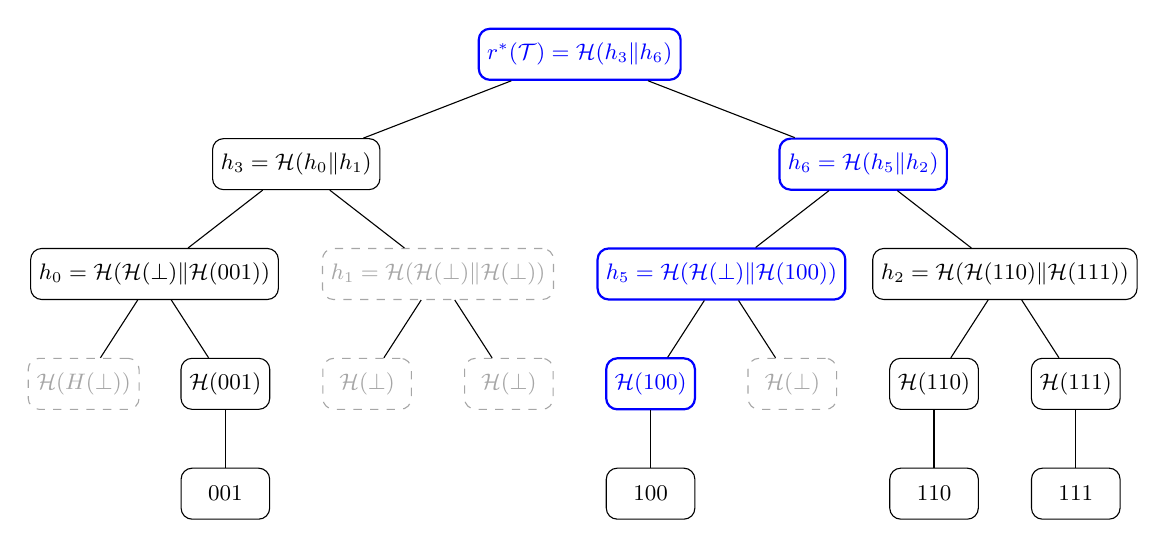
\begin{tikzpicture}[
		scale=0.9,
		transform shape,
		level distance=1.55cm,
		level 1/.style={sibling distance=8cm},
		level 2/.style={sibling distance=4cm},
		level 3/.style={sibling distance=2cm},
		every node/.style={
			draw, rectangle, rounded corners,
			align=center,
			minimum width=1.25cm,
			minimum height=0.72cm,
			font=\small
		},
		stored/.style={draw, opacity=1},
		pathnode/.style={
			draw, thick, blue, rectangle, rounded corners, align=center
		},
		implicit/.style={draw, dashed, opacity=0.35},
		edge from parent/.style={draw}
		]
		
		\node[stored,pathnode] {$r^*(\mathcal{T}) = \mathcal{H}(h_3 \Vert h_6)$}
		child { node[stored,] {$h_3 = \mathcal{H}(h_0 \Vert h_1)$}
			child { node[stored] {$h_0 = \mathcal{H}(\mathcal{H}(\bot) \Vert \mathcal{H}(001))$}
				child { node[implicit] {$\mathcal{H}(H(\bot))$}}
				child { node[stored] {$\mathcal{H}(001)$}
					child { node[stored] {$001$} }
				}
			}
			child { node[implicit] {$h_1 = \mathcal{H}(\mathcal{H}(\bot) \Vert \mathcal{H}(\bot))$}
				child { node[implicit] {$\mathcal{H}(\bot)$}}
				child { node[implicit] {$\mathcal{H}(\bot)$}}
			}
		}
		child { node[stored,pathnode] {$h_6 = \mathcal{H}(h_5 \Vert h_2)$}
			child { node[stored,pathnode] {$h_5 = \mathcal{H}(\mathcal{H}(\bot) \Vert \mathcal{H}(100))$}
				child { node[stored,pathnode] {$\mathcal{H}(100)$}
					child { node[stored] {$100$} }
				}
				child { node[implicit] {$\mathcal{H}(\bot)$}}
			}
			child { node[stored] {$h_2 = \mathcal{H}(\mathcal{H}(110) \Vert \mathcal{H}(111))$}
				child { node[stored] {$\mathcal{H}(110)$}
					child { node[stored] {$110$} }
				}
				child { node[stored] {$\mathcal{H}(111)$}
					child { node[stored] {$111$} }
				}
			}
		};
	\end{tikzpicture}
	\caption{Sparse Merkle Tree con el nodo $100$. Merkle Path de $100$ en azul.}
	\label{fig:update-sparse-merkle-tree-100-path}
\end{figure}

Se observa que nada nos impide combinar una Sparse Merkle Proof de exclusión y otra de inclusión para poder verificar la actualización correcta de un Sparse Merkle Tree. Esto nos será útil durante el trabajo.






